\subsubsection{} Обзор архитектуры iOS приложений
\label{sec:analysis:research:mobArch}

Любое современное мобильное приложение отображает динамически изменяемое содержимое, часто изменение одного поля модели способно повлечь за собой массу изменений в пользовательском интерфейсе. Важной проблемой при проектировании архитектуры мобильного приложения является консистентность состояния, данных и пользовательского интерфейса. Последние несколько лет сфера пытается уйти от императивного стиля программирования в сторону декларативного, для этого было разработано множество подходов, архитектур и инструментов. Одним из подходов является реактивное программирование и его конкретная имплементация -- \gls{rx}. Ниже будут рассмотрены традиционные подходы и инструменты, используемые при проектировании и имплементации архитектуры мобильного iOS приложения.

\paragraph {Apple MVC}
Классическим архитектурным паттером при разработке для платформы iOS является \gls{mvc}. Шаблон присваивает объектам в приложении одну из трех ролей: модель, представление или контроллер. Шаблон определяет не только роли объектов в приложении, но и способ взаимодействия объектов друг с другом. Каждый из трех типов объектов отделен от других абстрактными границами и связывается с объектами других типов через эти границы. Набор объектов определенного типа \gls{mvc} в приложении иногда называется слоем, например, слоем модели. \cite{apple:mvc} На рисунке \ref{sec:analysis:research:mobArch:apple-mvc:image:mvc} представлена связь между объектами паттерна \gls{mvc}.

\begin{figure}[h]
  \centering
    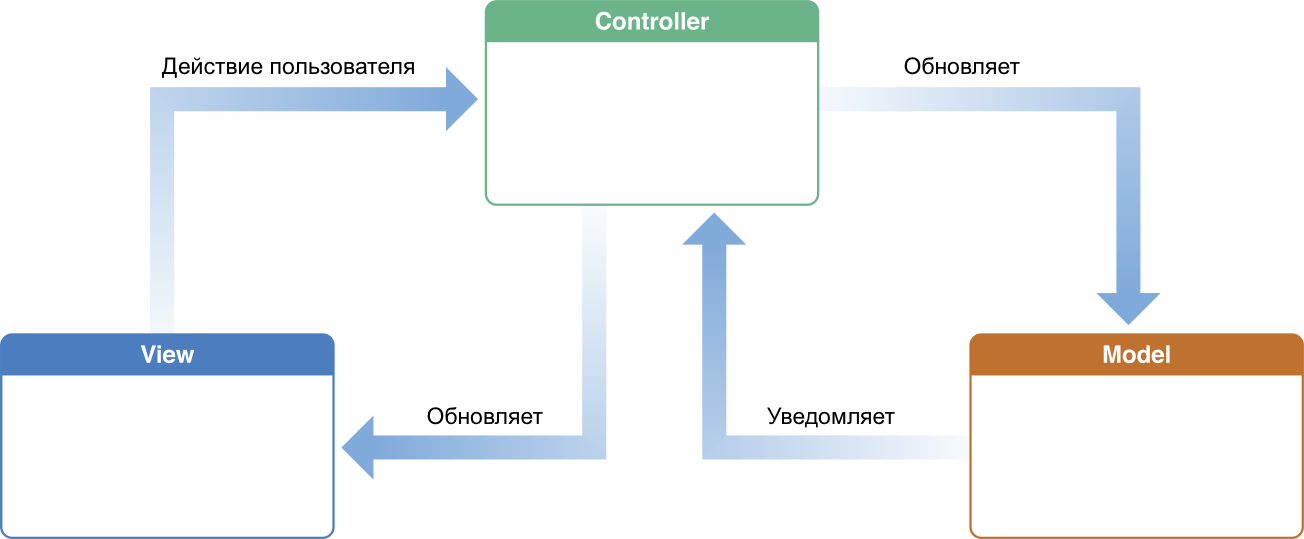
\includegraphics[width=1\textwidth]{inc/img/mvc.png}
  \caption{Связи между объектами MVC}
  \label{sec:analysis:research:mobArch:apple-mvc:image:mvc}
\end{figure}

\textbf{Объекты модели} инкапсулируют данные, специфические для приложения и описывают логику изменения этих данных. Для примера, объект модели может представлять персонажа в игре или контакт в книге контактов. Объекты модели могут иметь связь один ко многим или многие ко многим с остальными объектами модели, и поэтому иногда модельный уровень приложения представляет собой один или более объектных графов. В хорошей реализации паттерна объекты модели не должны иметь связи с объектами представления, изолируя данные от ошибок слоя презентации и действий пользователя: пользовательские действия в слое презентации, которые создают или модифицируют данные, влияют на модель при помощи промежуточного слоя котроллер и являются причиной создания или обновления объектов модели. Когда объект модели изменяется(например, новые данные были получены из сети), он уведомляет объект контроллера, который, в свою очередь, обновляет объект представления.

\textbf{Объектами представления} являются объекты, которые видит пользователь. Объекты данной группы умеют представлять себя графически на экране и реагировать на действия пользователя. Основной задачей объектов представления является вывести данные из модели приложения и позволить пользователю редактировать эти данные. Объекты представления часто обобщатся и используются между приложениями, хорошим примером такого переиспользования является \gls{uikit}. 

Объекты типа \textbf{котроллер} являются прослойкой между моделью и представлением, уведомляющих представление об изменениях в модели и наоборот. Объекты контроллера также могут выполнять настройку и координирование задач для приложения и управлять жизненными циклами других объектов. 

\paragraph {MVVM}
Шаблон \gls{mvvm} применяется при проектировании архитектуры приложения и позволяет разделить модель, представление и логику её представления. Первоначально был представлен сообществу Джоном Госсманом (John Gossman) в 2005 году как модификация шаблона Presentation Model. \cite{wiki:mvvm}

\gls{mvvm} является альтернативой паттерну \gls{mvc}. С паттерном \gls{mvvm} тесно связан паттерн <<связывание данных>>, позволяющий задать двухстороннюю связь между данными и отображением(сильно упрощая решение задачи динамически обновляемого контента). Шаблон состоит из трёх частей, связанных определённым образом: Model, View, ViewModel.

\textbf{Model}(Модель) представляет собой бизнес логику и фундаментальные данные, необходимые для работы приложения.

\textbf{View}(Представление) --- графический интерфейс, то есть окно, кнопки и так продолжая. Представление является подписчиком на события изменений значений свойств и пользователем команд, предоставляемых Моделью Представления.

\textbf{ViewModel}(Модель Представления) является прослойкой между Моделью и Представлением, предоставляя подготовленные для связывания данные из Модели и набор команд для изменения Модели Представлением.

Шаблон отвечает всем поставленным требованиям: является лёгким в использовании, позволяет разделить интерфейс на независимые компоненты, которые в будущем могут быть доработаны без необходимости дополнительных изменений в Представлении и имеет паттерны для динамического обновления данных. Исходя из этого было принято решение выбрать \gls{mvvm} в качестве основы для будущей архитектуры пользовательского интерфейса приложения.

\paragraph{}
\textbf{Функциональное программирование} --- раздел дискретной математики и парадигма программирования, в которой процесс выполнения трактуется как вычисление значений функций в математическом понимании последних (в отличие от функций как подпрограмм в процедурном программировании). Функциональное программирование предполагает обходиться вычислением результатов функций от исходных данных и результатов других функций, и не предполагает явного хранения состояния программы. Соответственно, не предполагает оно и изменяемость этого состояния. \cite{wiki:fp}

После прочтения определения функционального программирования становится очевидно, что использовать исключительно этот подход при построении интерактивного приложения с пользовательским интерфейсом является крайне сложной задачей. В приложениях данного типа состояние навязывается и требованиями и операционной системой. Тем не менее существует ряд функциональных подходов, соблюдение которых значительно понижает количество ошибок:

\begin{itemize}
\item Отсутствие глобального состояния;
\item Отсутствие изменяемого состояния;
\item Чистые функции;
\item Функции высших порядков;
\item Рекурсия.
\end{itemize}

После обобщения и ослабления некоторых признаков, были выведены следующие принципы будущей архитектуры:

\begin{enumerate}
\item \textit{Сокращение глобального состояния}. Данный пункт не подразумевает полный отказ от глобального состояния, однако призывает как можно больше данных передавать при инициализации, параметрами методов или в виде \gls{observable}.
\item \textit{Модульность}. Концепция чистой функции позволяет трактовать программу, как результат применения цепочки функций, следовательно всё приложение(и его отдельные части) можно декомпозировать на множество чистых функций, что позволяет повысить тестируемость и побуждает избегать неявных зависимостей.
\item \textit {Аккуратное использование изменяемого состояния}. Данный принцип призывает делать выбор в пользу неизменяемых типов данных, передаваемых по значению. 
\item \textit {Ответственный дизайн типов}. Функциональная программа с хорошим дизайном крайне трепетно относится к используемым типам, описывая ими все возможные побочные эффекты и структурируя код. Огромное количество ошибок разработчика обнаруживается на стадии компиляции.
\end{enumerate}

К сожалению, компилятор языка Swift не гарантирует оптимизацию хвостовой рекурсии, поэтому от идеи повсеместного использования рекурсии было решено отказаться в пользу богатого набора функций высшего порядка в стандартной библиотеке. В пункте \ref{practice:instruments:swift} будут раскрыты особенности языка Swift, которые помогают эффективно использовать описанные выше принципы, такие как \gls{cow}, функции высшего порядка, замыкания, Optional и некоторые другие.